\section{The Large Hadron Collider} \label{sec:LHC}

The Large Hadron Collider is a particle accelerator located about 100 meters underground, straddling the border of France and Switzerland. It is the largest machine ever built, and an aerial view is shown in Fig \ref{fig:LHC_BirdsEye}, including the positions of the major experiments it delivers collisions to: The ALICE, ATLAS, CMS, and LHCb detectors. Its construction took place from 1998 to 2008, with the intention of building a machine which can produce proton-proton collisions at a center of mass energy not yet achieved, where part of its physics program was to experimentally discover the Higgs boson, and enhance the ability to test a variety of beyond the standard model (BSM) theories. 

\begin{figure}[H]
    \centering
    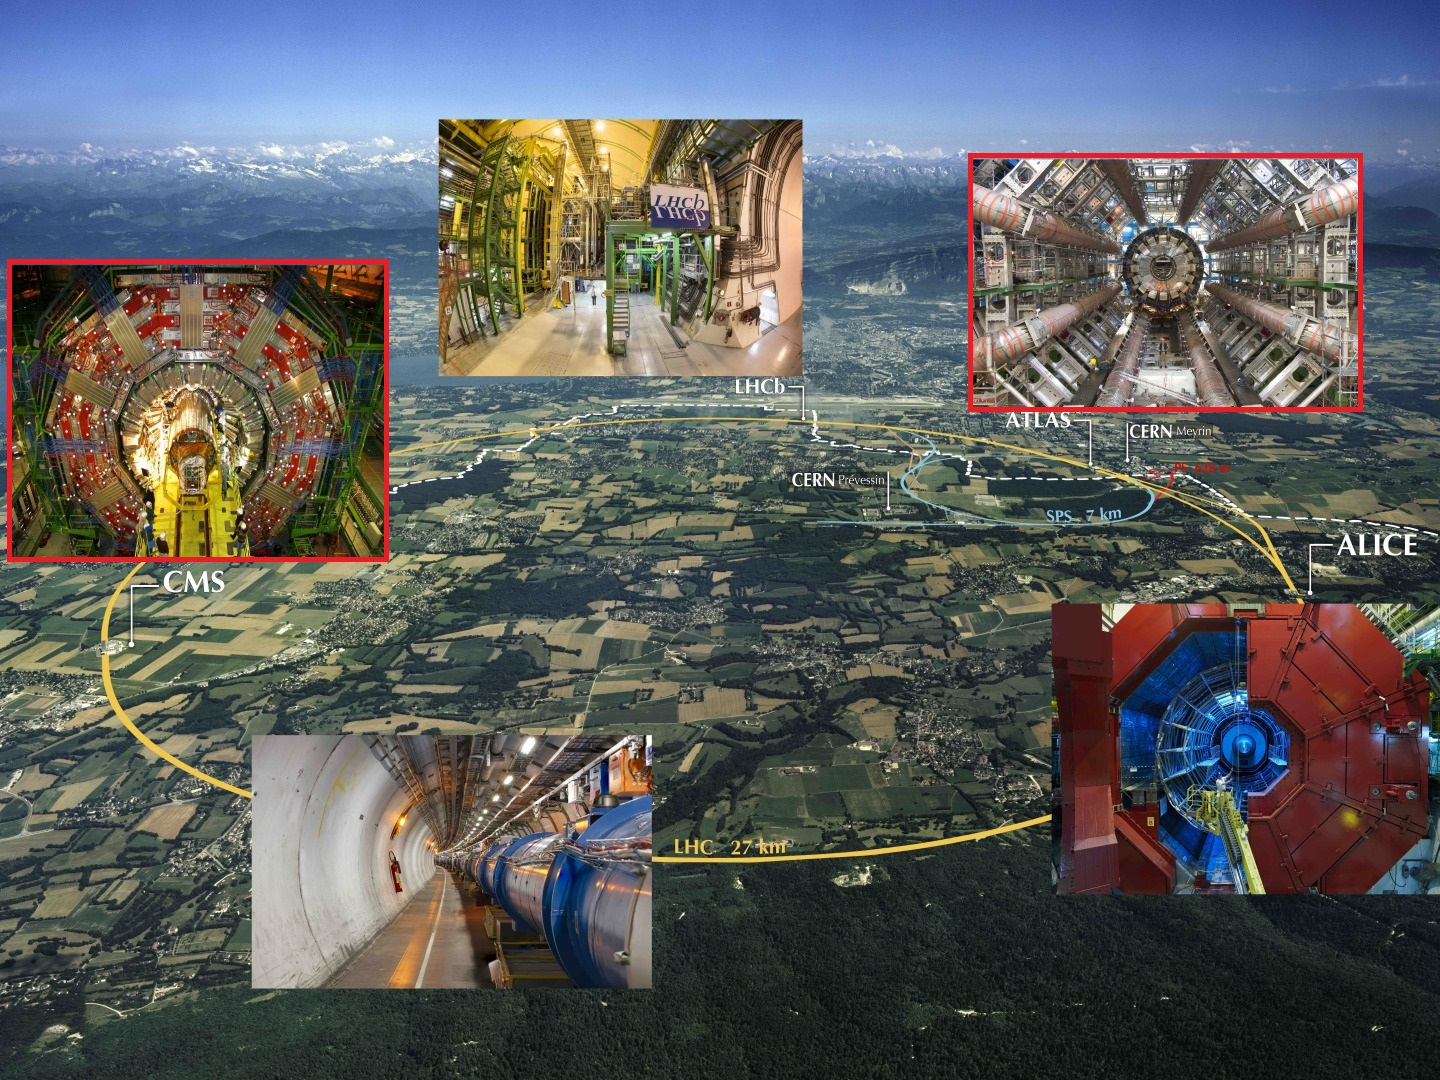
\includegraphics[width=\textwidth]{Images/LHC/LHCCollage_withExperiments.jpeg}
    \caption{The geographical location of the Large Hadron Collider (yellow solid), relative to the French-Swiss border (white dashed) and LHC experiments (white labels)}
    \label{fig:LHC_BirdsEye}
\end{figure}

The LHC is the final acceleration stage in a complex of linear and circular accelerators, all of which are depicted in Figure \ref{fig:CERN_Acc_Complex}. 

\begin{figure}[H]
    \centering
    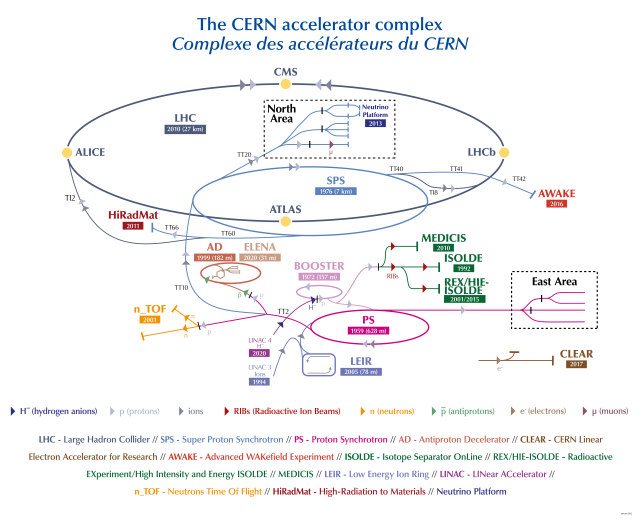
\includegraphics[width=\textwidth]{Images/LHC/CERN_Accelerator_Complex.png}
    \caption{CERN accelerator complex}
    \label{fig:CERN_Acc_Complex}
\end{figure}

% https://www.lhc-closer.es/taking_a_closer_look_at_lhc/0.proton_source
% https://home.cern/science/accelerators/proton-synchrotron-booster
% https://home.cern/science/accelerators/proton-synchrotron
% https://home.cern/science/accelerators

Proton-proton collisions are a useful basis for performing a variety of particle physics analyses, as with a high enough initial energy, all of the SM fermions and bosons can be produced. As the mass of the proton is small compared to that of other SM particles such as the W and Z bosons (about 1/90th) or the Higgs boson (about 1/125th the mass), particle accelerators are used in order to increase the energy of the protons such that this energy can be converted into these more massive particles. Also as seen in the theoretical background chapter, higher center-of-mass energies can lead to higher likelihoods of producing rare processes, such as Higgs pair production. 

In Figure \ref{fig:LHC_Long_Term_Schedule}, the long term schedule of the LHC is shown. It should be noted that this schedule is always subject to change, as unforeseen circumstances may come up during this long time period.

% At the end of LHC Run 3, the LHC will enter Long Shutdown 3 (LS3), where the LHC will be upgraded to the High Luminosity LHC (HL-LHC). The LHC long term schedule, which is subject to change, is shown in Figure \ref{fig:LHC_Long_Term_Schedule}.

\begin{figure}[H]
    \centering
    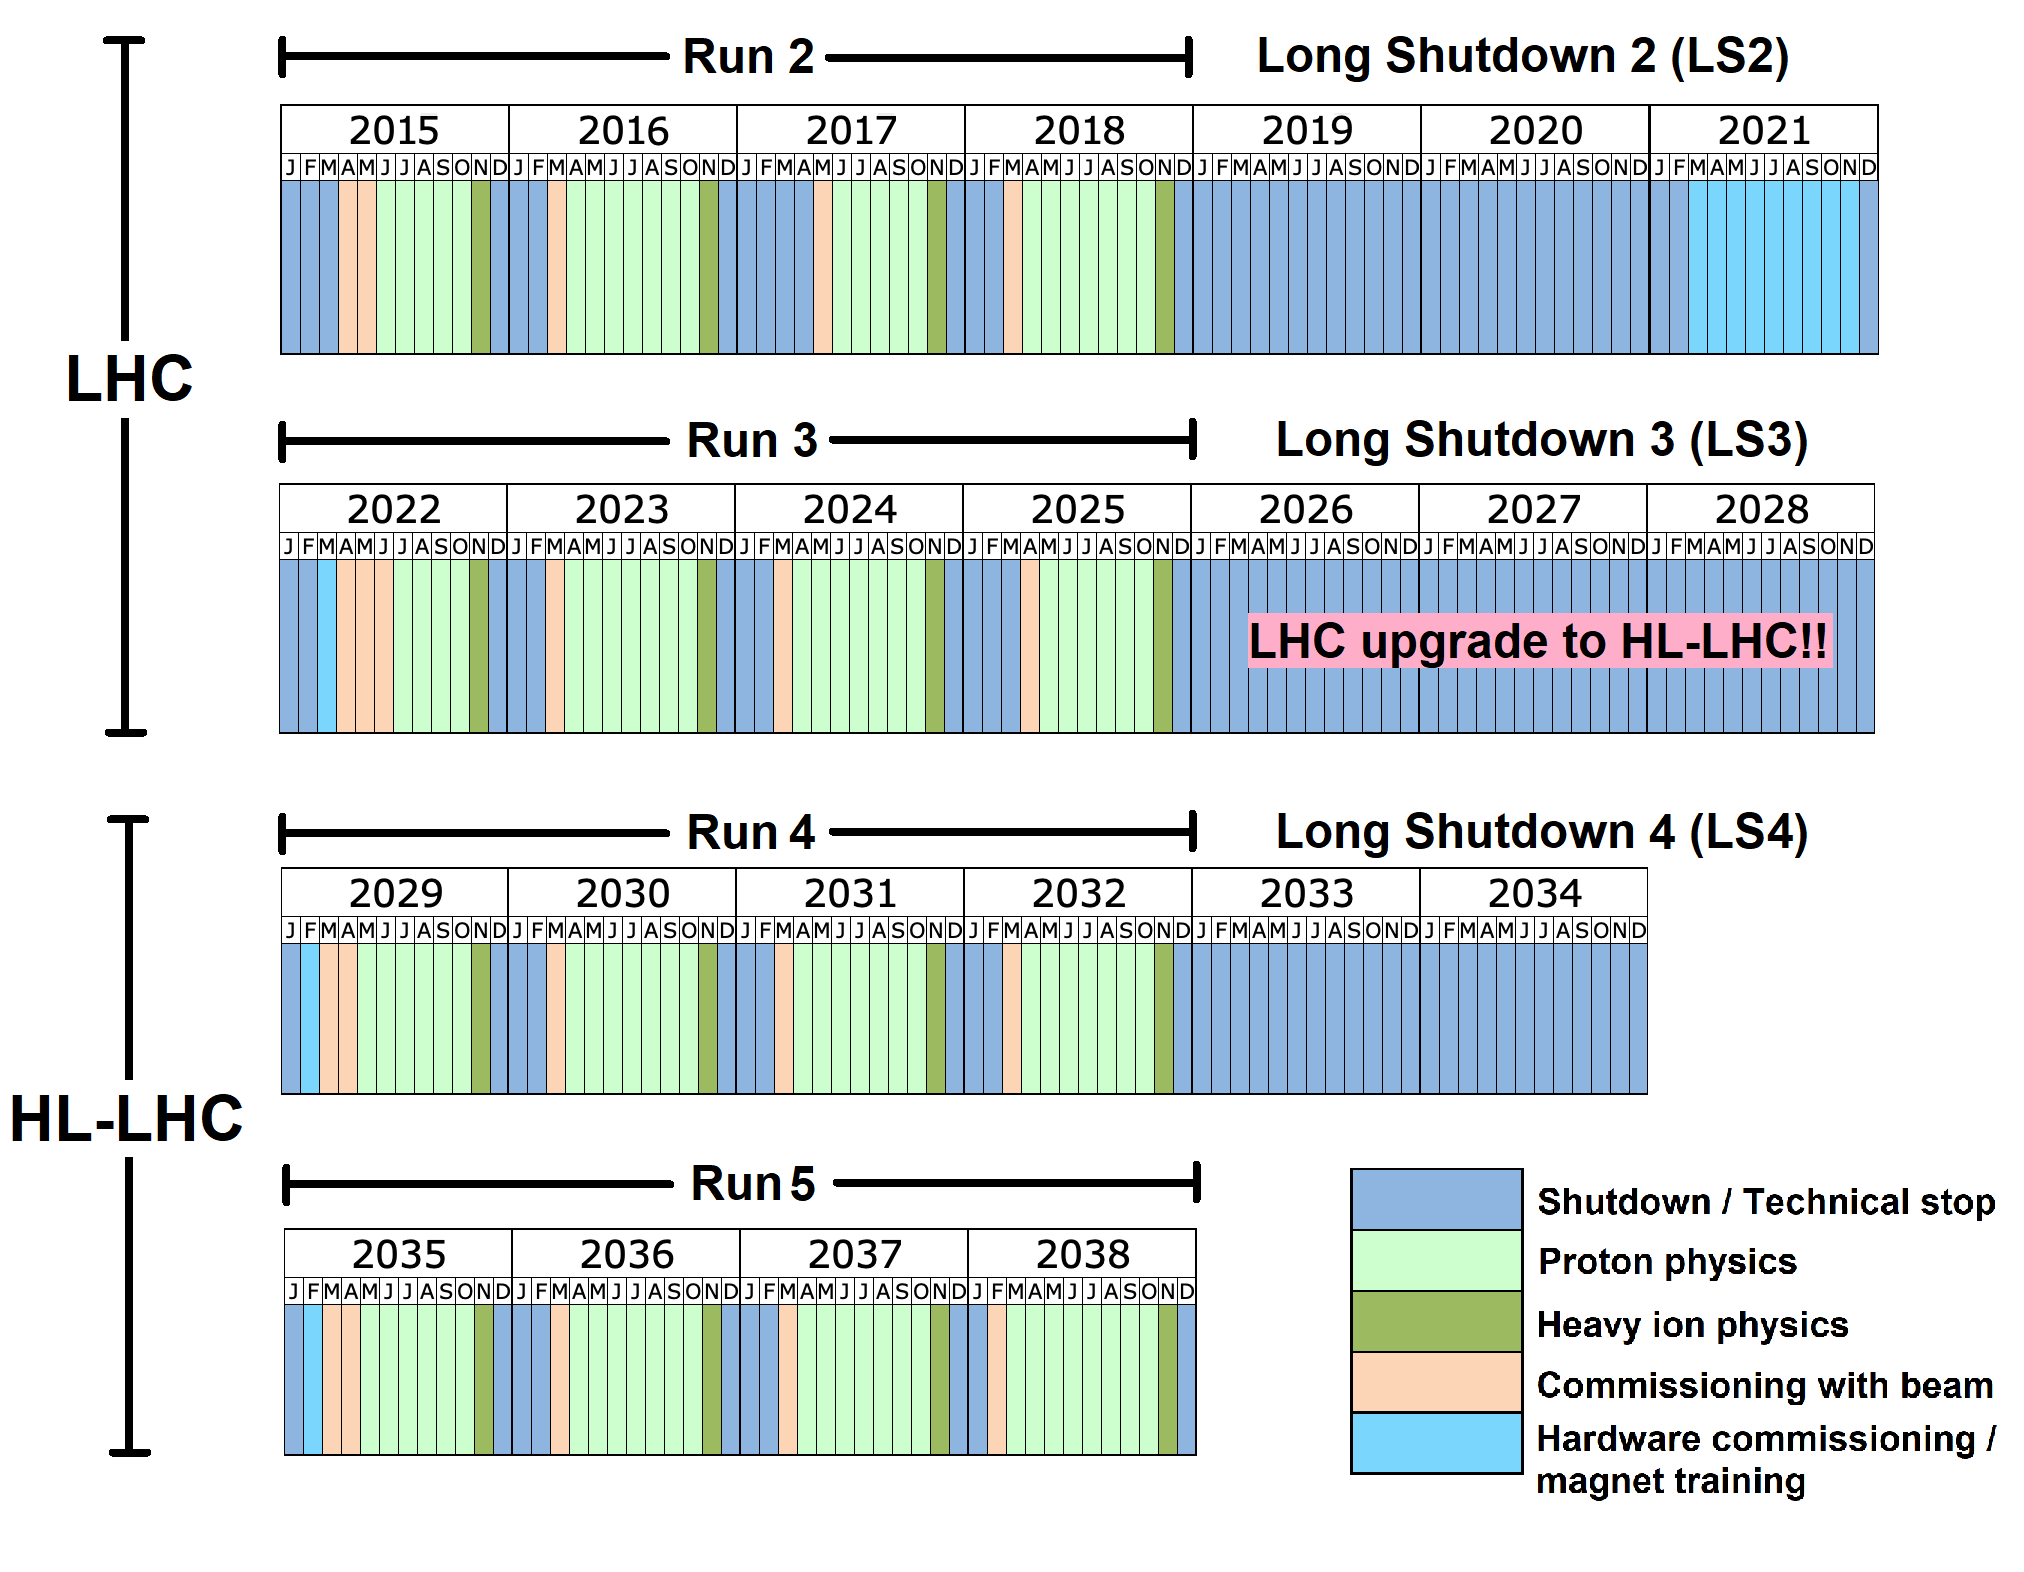
\includegraphics[width=\textwidth]{Images/LHC/LHC_LongTermSchedule_MyVersion.png}
    \caption{LHC long term schedule}
    \label{fig:LHC_Long_Term_Schedule}
\end{figure}

\subsection{Run 2}

Run 2 of the LHC took place from 2015-2018 as shown in Figure \ref{fig:LHC_Long_Term_Schedule}, where very little data was delivered to the experiments in 2015, and therefore the vast majority of Run 2 analyses include data collected from 2016-2018. 

In order to prepare proton-proton collisions with a high center of mass energy and instantaneous luminosity, during LHC Run 2 the CERN accelerator complex began with a source of H$_{2}$, a hydrogen gas. This H$_{2}$ gas was injected into a cavity in the presence of an electric field in order to strip it of its electrons, yielding a pure proton source. These protons were then sent to LINAC 2 (Linear Accelerator 2) to perform an initial acceleration of protons to an energy of 50 MeV. The proton beam then enters the Proton Synchrotron Booster, where they are further accelerated to 1.4 GeV for injection into the Proton Synchrotron, where the beam is further accelerated to 26 GeV. The penultimate stop in the proton beams' acceleration journey is the Super Proton Synchrotron (SPS). In SPS, proton are accelerated up to 450 GeV each and are then injected into the LHC. It is in the LHC where the proton beams, during Run 2, were accelerated up to 6.5 TeV each corresponding to a center of mass energy of 13 TeV, then a world record. 

Each stage of acceleration is performed thanks to a variety of superconducting magnets and radio-frequency cavities, with additional magnets used to focus the beams.

During LHC Run 2, the LHC delivered about 156 fb$^{-1}$ of proton-proton collisions to the CMS and ATLAS experiments, with a average number of simultaneous collision interactions, known as pile-up, around 36. 

% https://twiki.cern.ch/twiki/bin/view/AtlasPublic/LuminosityPublicResultsRun2

\subsection{Run 3}

Run 3 of the LHC is expected to last from 2022-2025, as shown in Figure \ref{fig:LHC_Long_Term_Schedule}. During LHC Run 3, the acceleration stages will generally be the same as during LHC Run 2, but with the replacement of LINAC 2 in favor of LINAC 4. 

On July 5th 2022, the LHC delivered its first ``stable beam" collisions at a new world record center-of-mass energy: 13.6 TeV, corresponding to beam energies of 6.8 TeV each, displayed on the LHC monitor shown in Figure \ref{fig:LHCMonitor_first13p6TeV}. 

\begin{figure}[H]
    \centering
    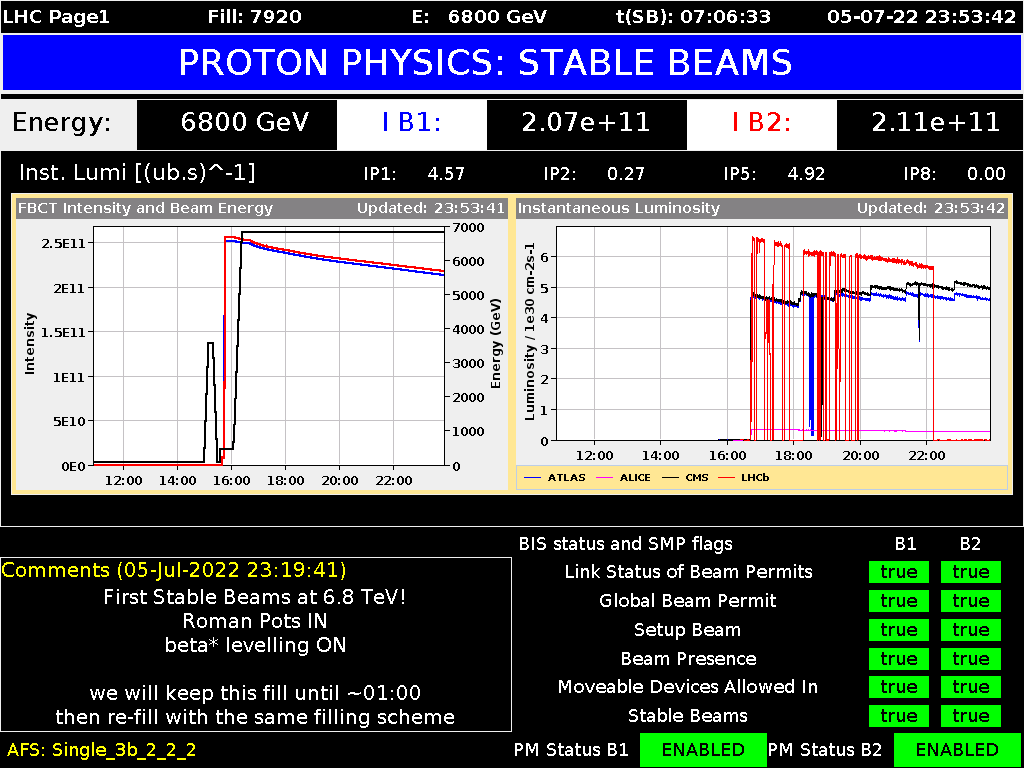
\includegraphics[width=\textwidth]{Images/LHC/First_13p6TeV_Collisions.png}
    \caption{LHC monitor during the first stable beams collisions at $\sqrt{s} = 13.6$ TeV}
    \label{fig:LHCMonitor_first13p6TeV}
\end{figure}

This marked the official start of LHC Run 3. The LHC will spend July 2022 increasing the number of proton bunches in the machine, and starting around the end of July 2022 and early August 2022, will have a full machine of proton bunches in order to provide high intensity collisions to the experiments so that large amounts of data can be recorded.

During LHC Run 3, it is expected that the average pileup will be around 55 simultaneous interactions per bunch crossing, and early estimates of total integrated luminosity are about double that delivered during Run 2. Due to this increase in pileup and total radiation dose to the detectors, it will be important to continue to optimize the LHC detectors during Run 3 to ensure quality data is taken. 

\subsection{The High-Luminosity LHC}

At the end of LHC Run 3, the LHC will enter Long Shutdown 3 (LS3), during which the LHC will be upgraded to the High Luminosity LHC (HL-LHC). The HL-LHC is then planned to deliver record amounts of collisions data to the experiments over Runs 4 and 5 between the years 2029-2038, as shown in Figure \ref{fig:LHC_Long_Term_Schedule}. 

The sensitivity and uncertainty of a plethora of physics analyses is driven by the yields, or number of events, of the analyzed dataset. Increasing the number of events of the available data to be used for analysis is one of the main motivations for upgrading the LHC, allowing for a higher integrated luminosity which will lead to more sensitive BSM searches, and more precise SM measurements. 

The HL-LHC expects to deliver an unprecedented 3000 fb$^{-1}$ to the main LHC experiments, which will make up about 90\% of the experiments' total datasets. A visualization of the integrated luminosity to be delivered by the LHC and HL-LHC over time, with a slightly shifted timeline, is shown in Figure \ref{fig:LHC_Int_Lumi}.

\begin{figure}[H]
    \centering
    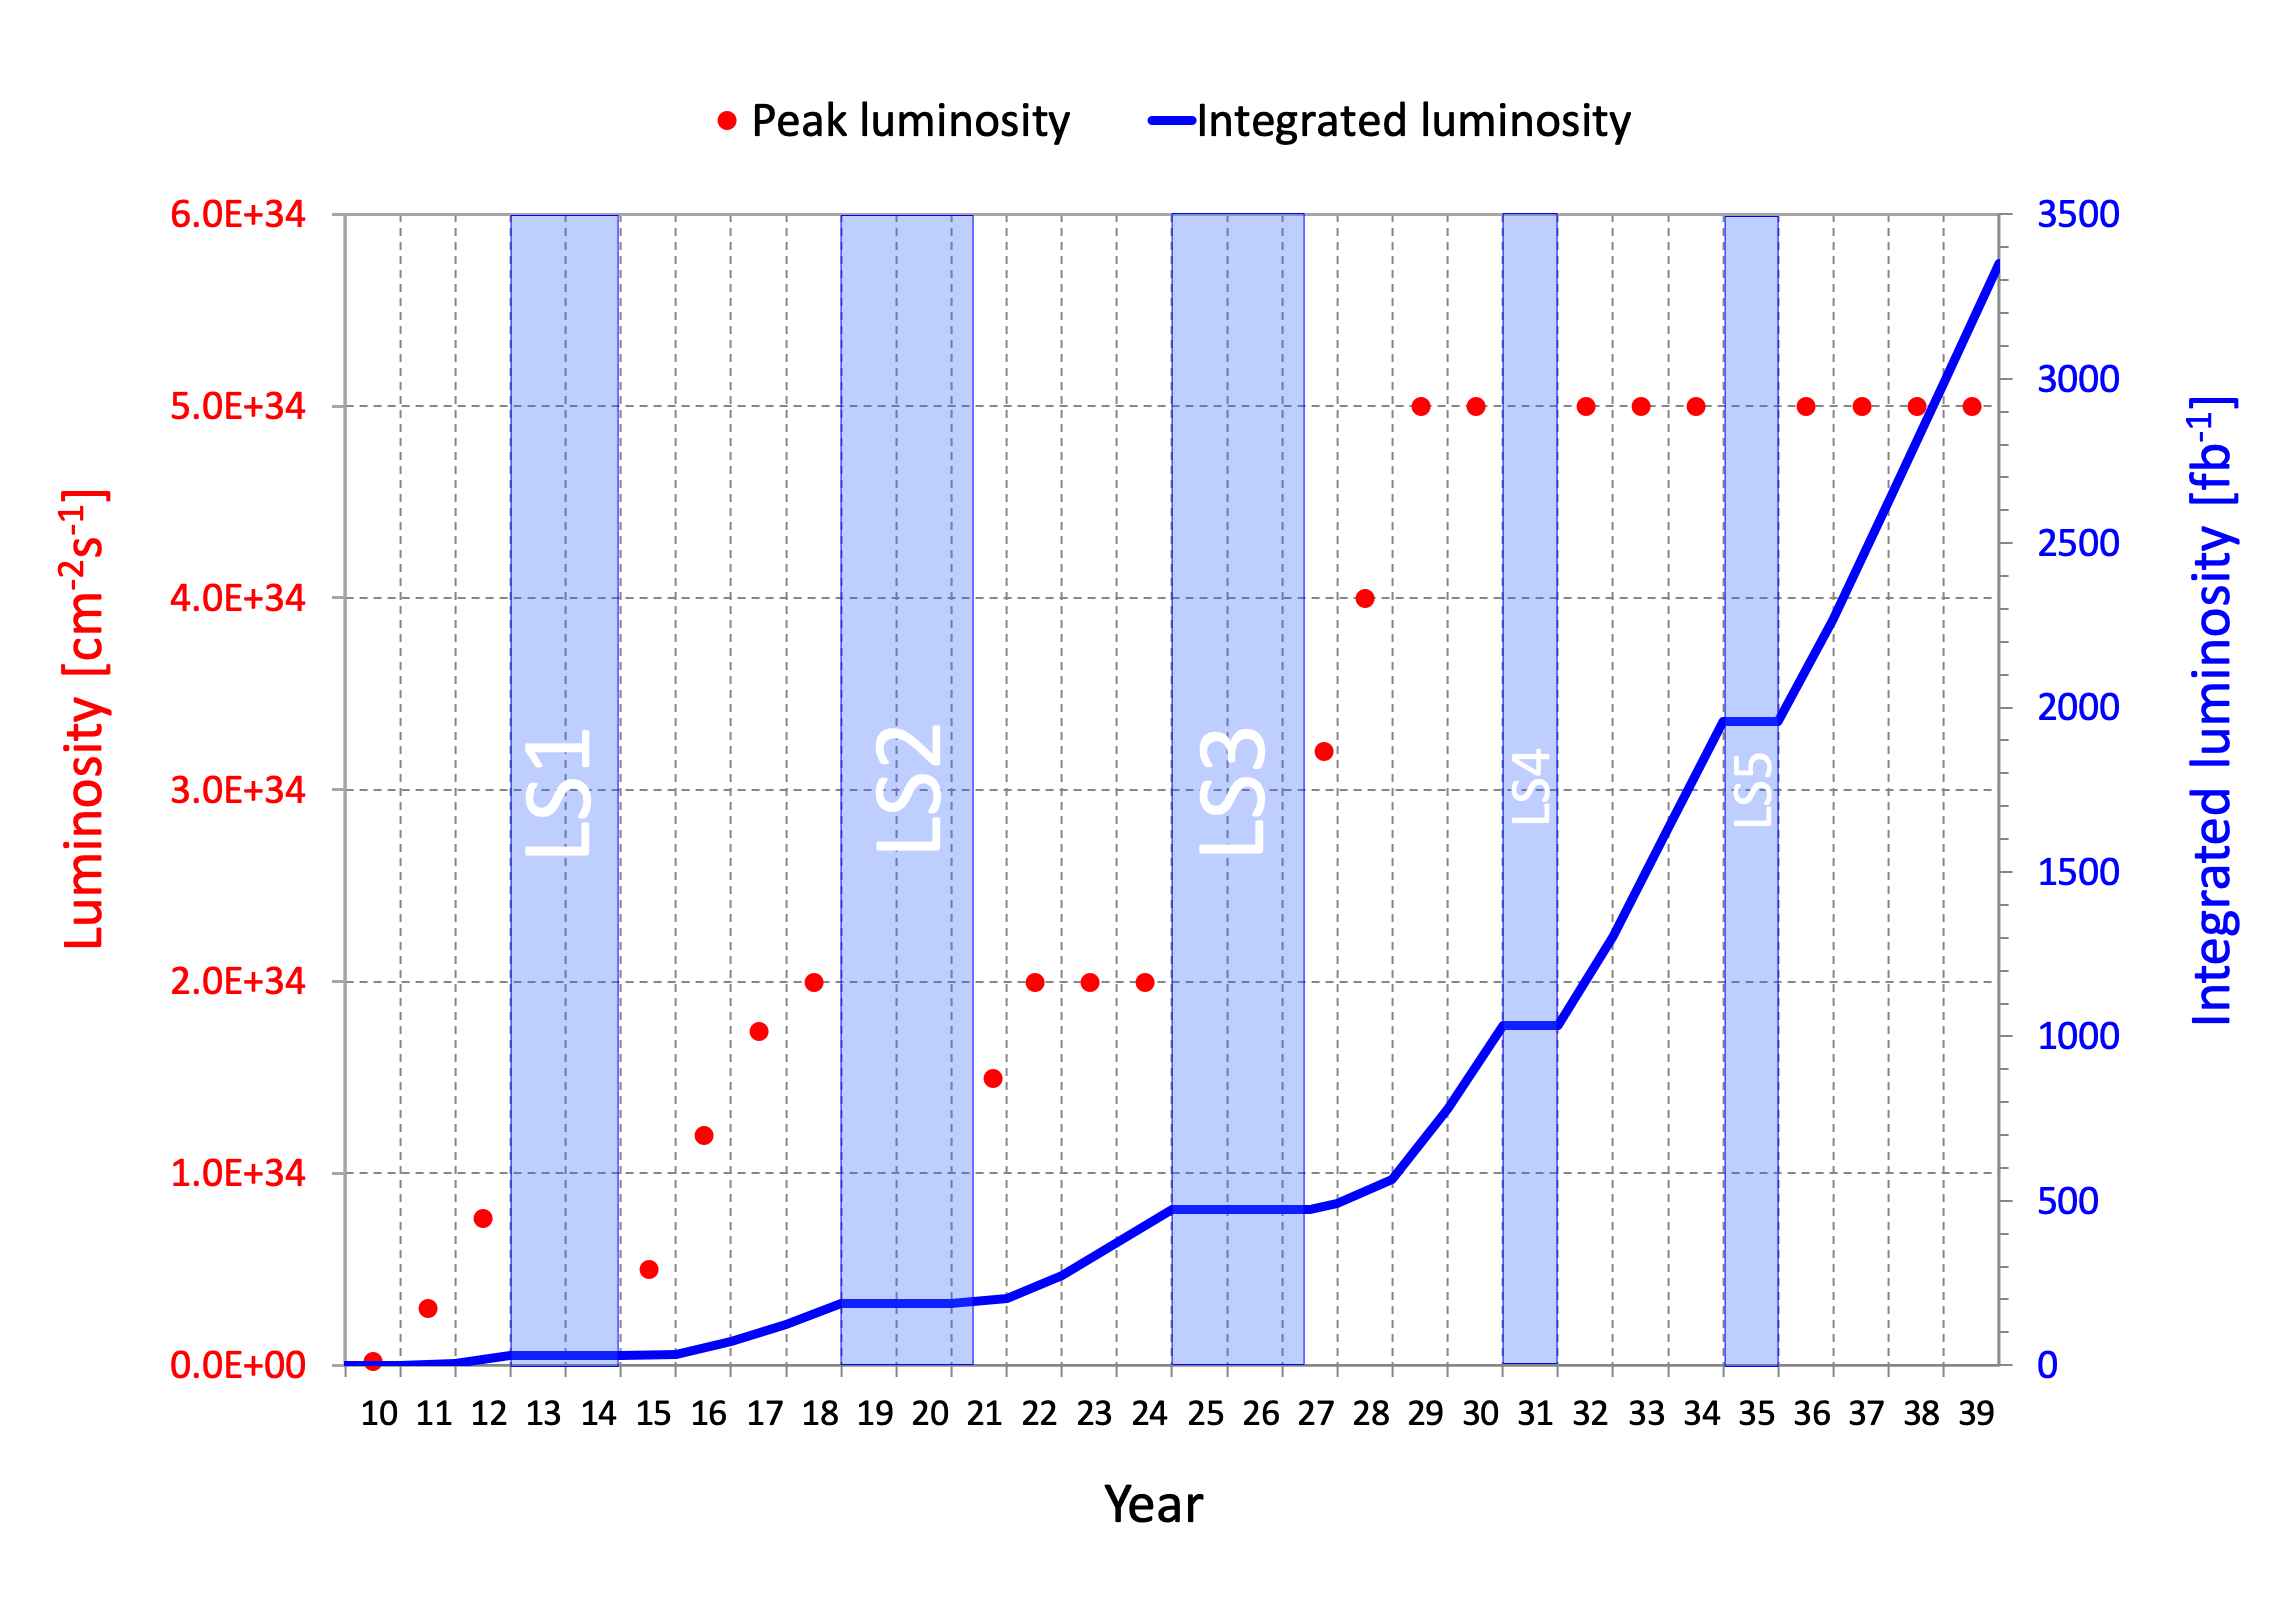
\includegraphics[width=\textwidth]{Images/LHC/LHC-nom-lumi-proj-with-ions.png}
    \caption{LHC and HL-LHC expected integrated luminosity over time} % https://lhc-commissioning.web.cern.ch/schedule/images/LHC-nom-lumi-proj-with-ions.png
    \label{fig:LHC_Int_Lumi}
\end{figure}

While the upgraded HL-LHC will deliver extremely large datasets to the experiments, this will also lead to very challenging data-taking conditions: One aspect will be the increased pileup which will be produced during HL-LHC collisions, expected to increase from about 55 simultaneous interactions during Run 3 data-taking, to about 140 during HL-LHC. This means that while more interesting signal-like interactions may occur during this data-taking period, there will be many more less-interesting background interactions which will need to be separated from signal interactions. Additionally, during this period detectors will receive a very large amount of radiation which will degrade their sub-detectors. In order to deal with the increase in pileup and radiation, the LHC experiments plan to implement major upgrades so that they can collect high quality data during HL-LHC in order to extend their BSM reaches and SM measurement precisions. 